\section{Prototype work}\label{sprint-3-prototypes}
For this sprint, we have refactored a few of the older prototypes and also created some new ones for the new user stories.

\subsection{New timer and week plan template}
We refactored the timer on the show activity screen to use the common GIRAF buttons so that we can keep a consistent design. The figure to the right shows a screen for selecting a template when creating a new week plan.
\begin{figure}[H]
    \begin{subfigure}{0.5\textwidth}
    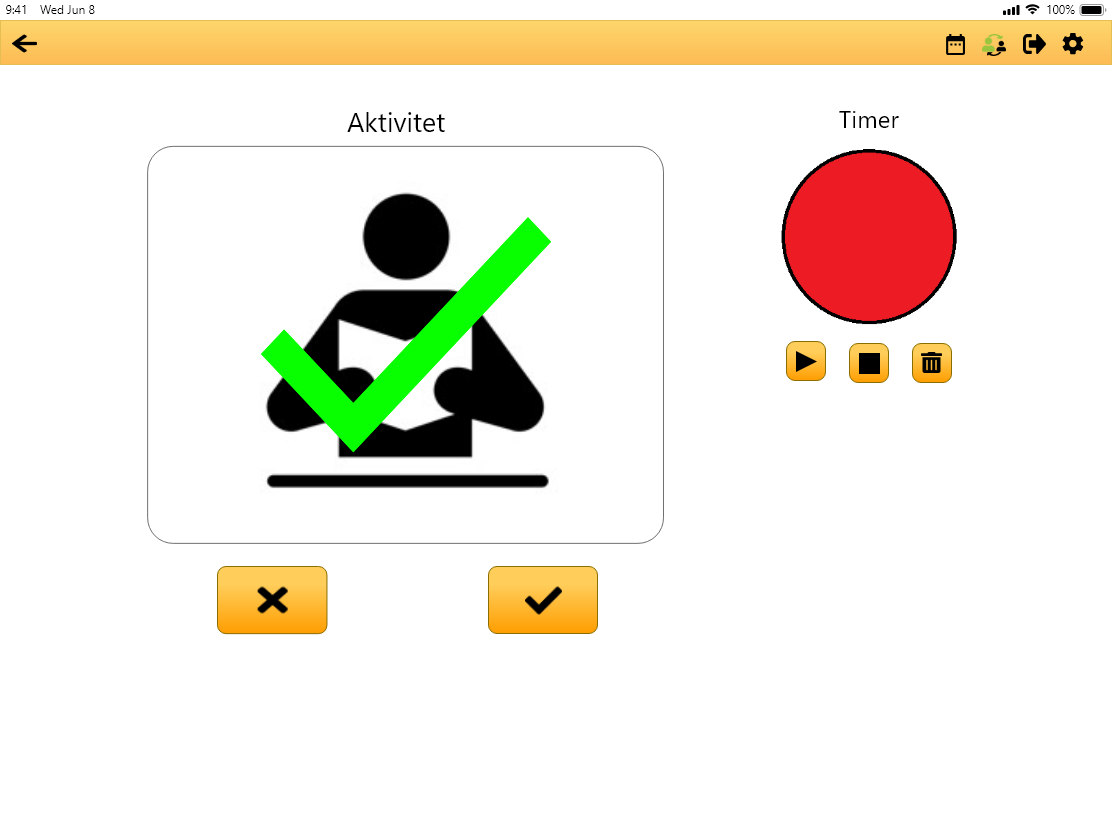
\includegraphics[width=1\linewidth, height=5cm]{aktivitet_new_timer.png}
    \caption{New timer for activity}
    \label{fig:activity_new_timer}
    \end{subfigure}
    \begin{subfigure}{0.5\textwidth}
        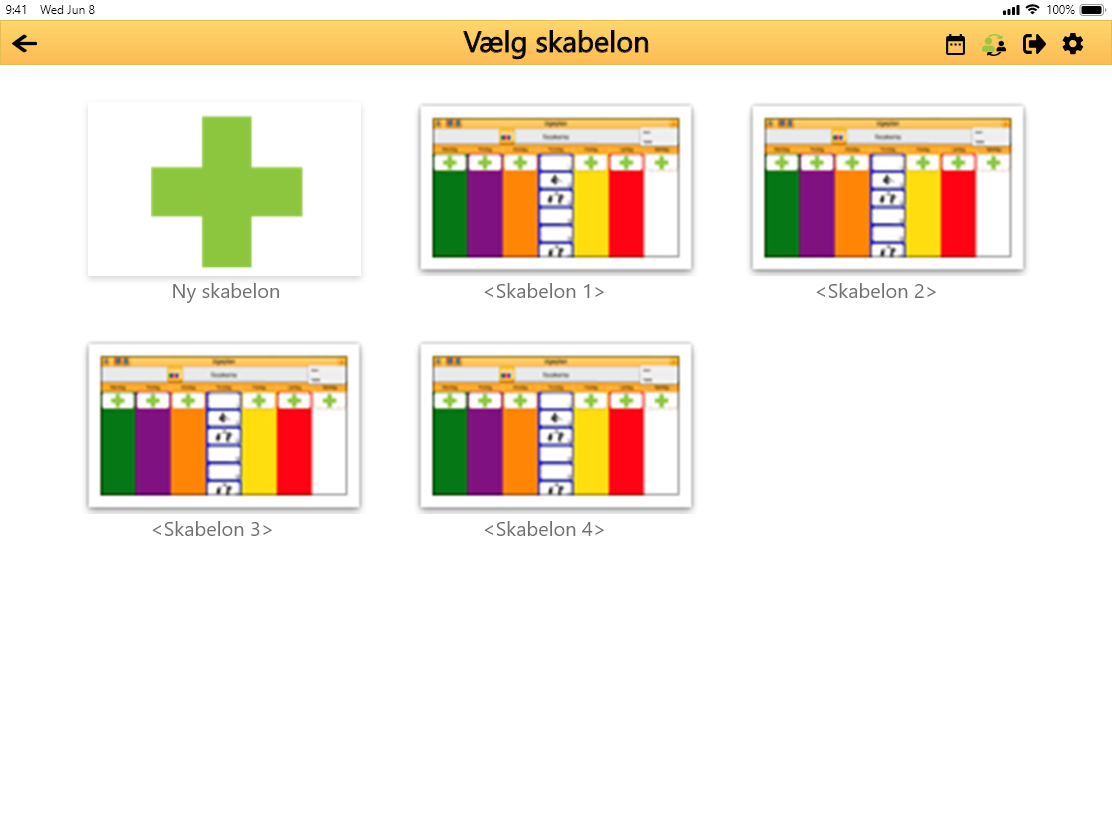
\includegraphics[width=1\linewidth, height=5cm]{ugeplan_skabelon.png}
    \caption{Week plan template select screen}
    \label{fig:weekplan_template_screen}
    \end{subfigure} 
    \caption{}
    \label{activity_new_timer_and_weekplan_template_screen}
\end{figure}

\subsection{Setting pages}
We created a number of prototypes for the settings pages. Here we show two of them where the first is the overall view of the settings, and the second one shows the settings screen where the guardian can select a color theme for the week plan.
\begin{figure}[H]
    \begin{subfigure}{0.5\textwidth}
    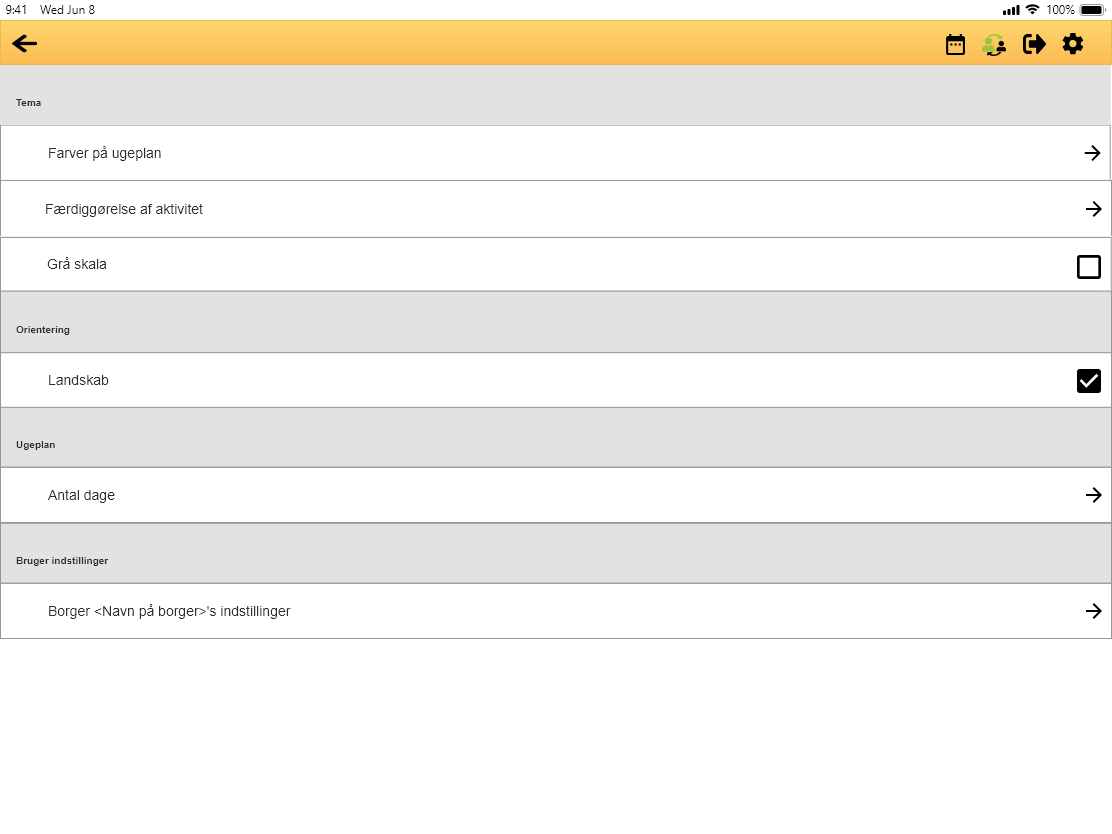
\includegraphics[width=1\linewidth, height=5cm]{Indstillinger.png} 
    \caption{Setting page}
    \label{fig:settings}
    \end{subfigure}
    \begin{subfigure}{0.5\textwidth}
        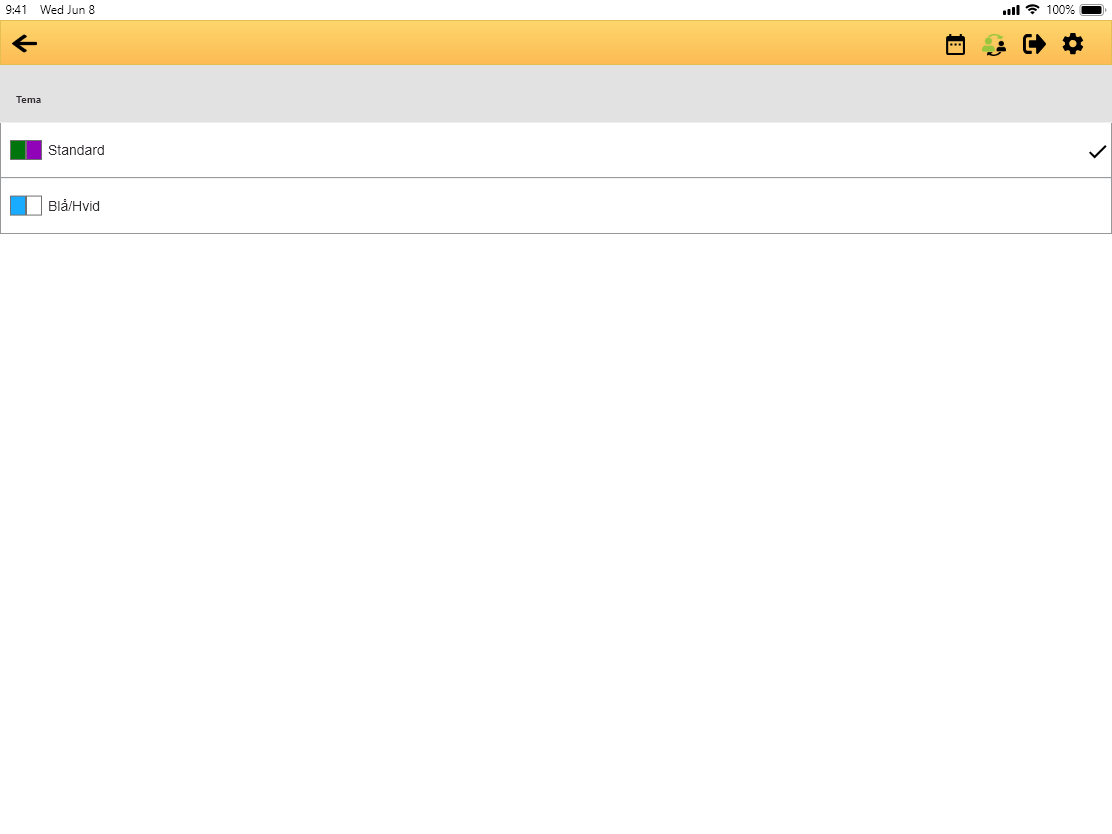
\includegraphics[width=1\linewidth, height=5cm]{indstillinger_ugeplan_farver.png}
    \caption{Settings page for week plan color choice}
    \label{fig:settings_color_choice}
    \end{subfigure}
    \caption{} 
    \label{settings_and_settings_color_choice}
\end{figure}

\subsection{Copy week plan}
We refactored the prototypes for copying a week plan to other citizens to include the new dialog boxes to make the design consistent. In \autoref{fig:copy_weekplan} we see a confirm dialog for copying a week plan. In \autoref{fig:copy_weekplan_confirm_copy} we see the screen for choosing which citizens the week plan should be copied to. 
\begin{figure}[H]
    \begin{subfigure}{0.5\textwidth}
    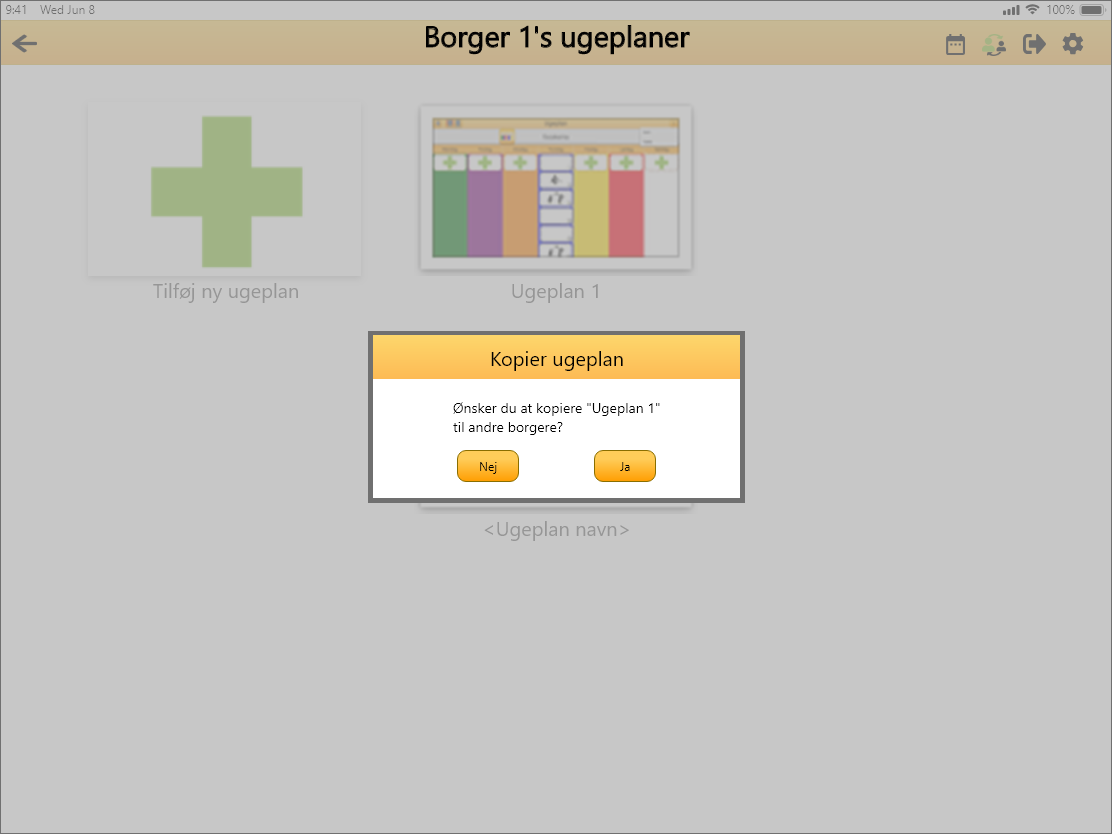
\includegraphics[width=1\linewidth, height=5cm]{copy_weekplan.png} 
    \caption{Copy week plan dialog}
    \label{fig:copy_weekplan}
    \end{subfigure}
    \begin{subfigure}{0.5\textwidth}
        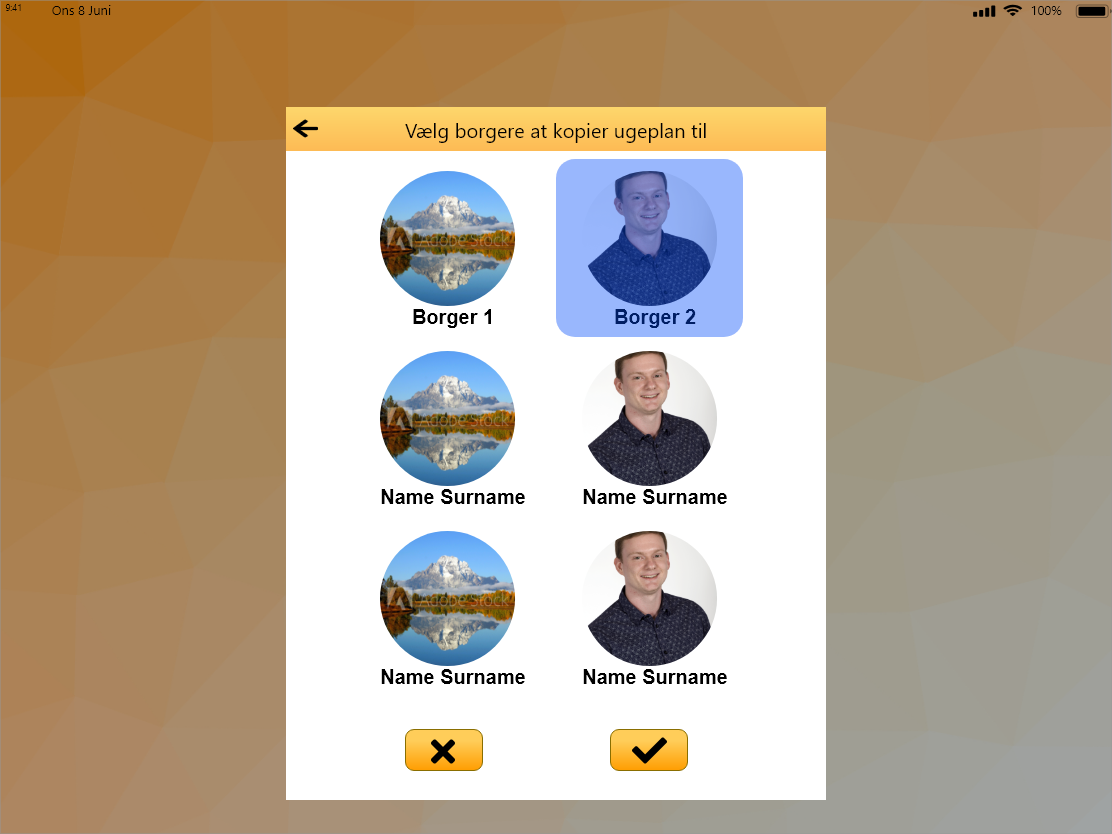
\includegraphics[width=1\linewidth, height=5cm]{copy_weekplan_confirm_copy.png}
    \caption{Choose citizens to copy week plan to and confirm}
    \label{fig:copy_weekplan_confirm_copy}
    \end{subfigure} 
    \caption{}
    \label{fig:copy_weekplan_confirm_copy_and_copy_weekplan}
\end{figure}
\noindent
Finally, in \autoref{fig:copy_weekplan_confirmed} we see the confirmation dialog when the week plan is successfully copied.

\begin{figure}
    \centering
    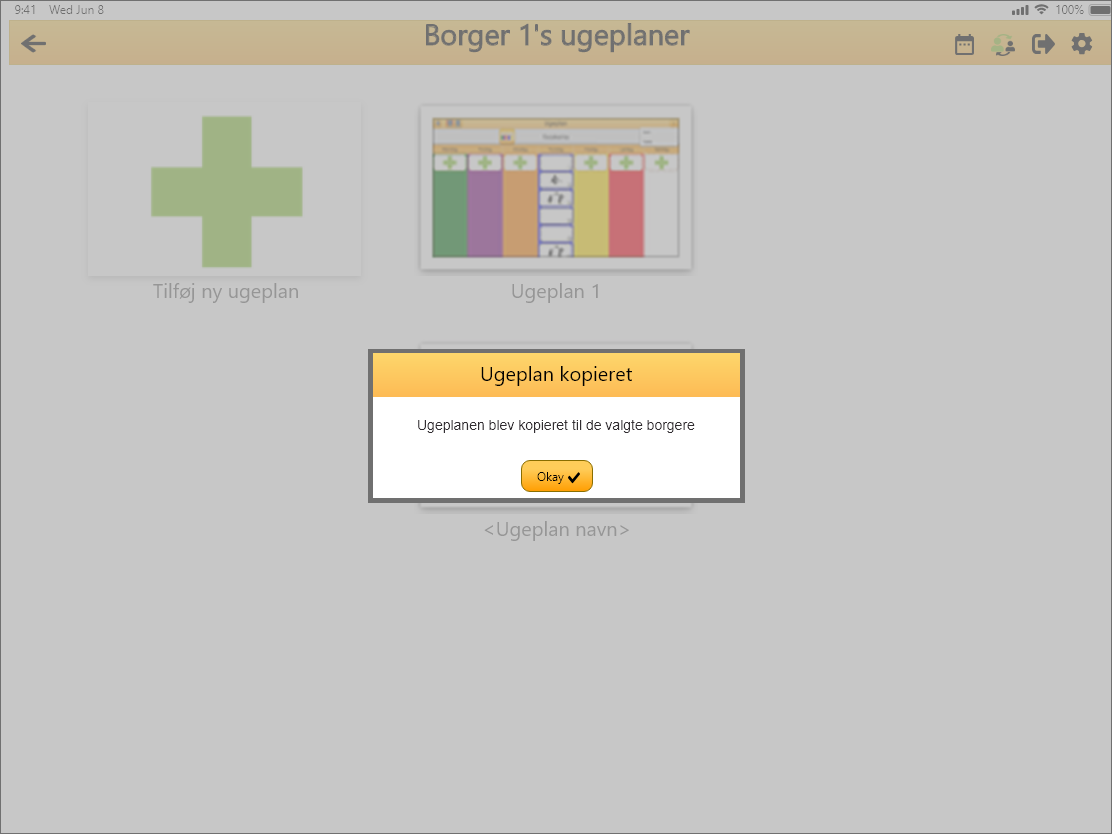
\includegraphics[width=0.5\linewidth]{copy_weekplan_confirmed.png} 
    \caption{Week plan copied confirmation screen}
    \label{fig:copy_weekplan_confirmed}
\end{figure}

\subsection{Copying of activities}
Here we created two different versions of prototypes that show how activities are copied between weekdays. This is because we were unsure of what the customer would like so we created different versions to show them. The dialog with the checkboxes have the advantage of being able to copy to more than one day at a time.
\begin{figure}[H]
    \begin{subfigure}{0.5\textwidth}
    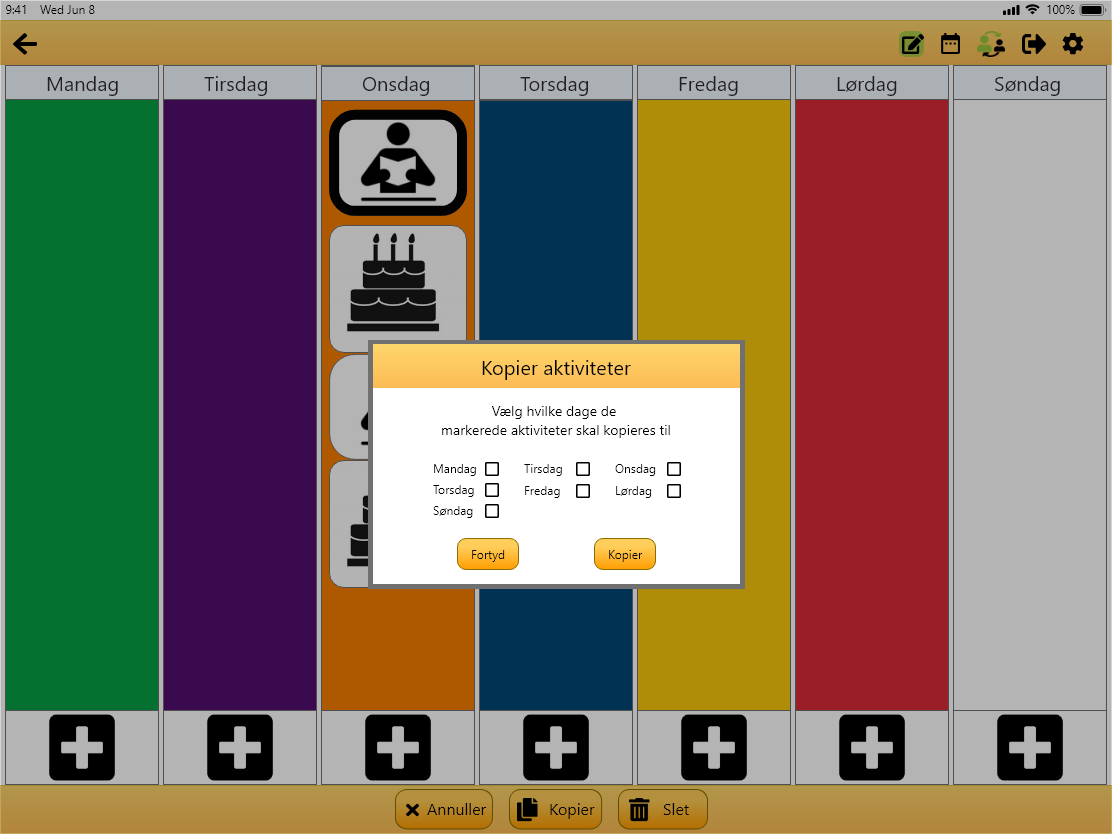
\includegraphics[width=1\linewidth, height=5cm]{mark_mode_copy_checkbox.png} 
    \caption{Copy activities dialog with checkboxes}
    \label{fig:mark_mode_copy_checkbox}
    \end{subfigure}
    \begin{subfigure}{0.5\textwidth}
        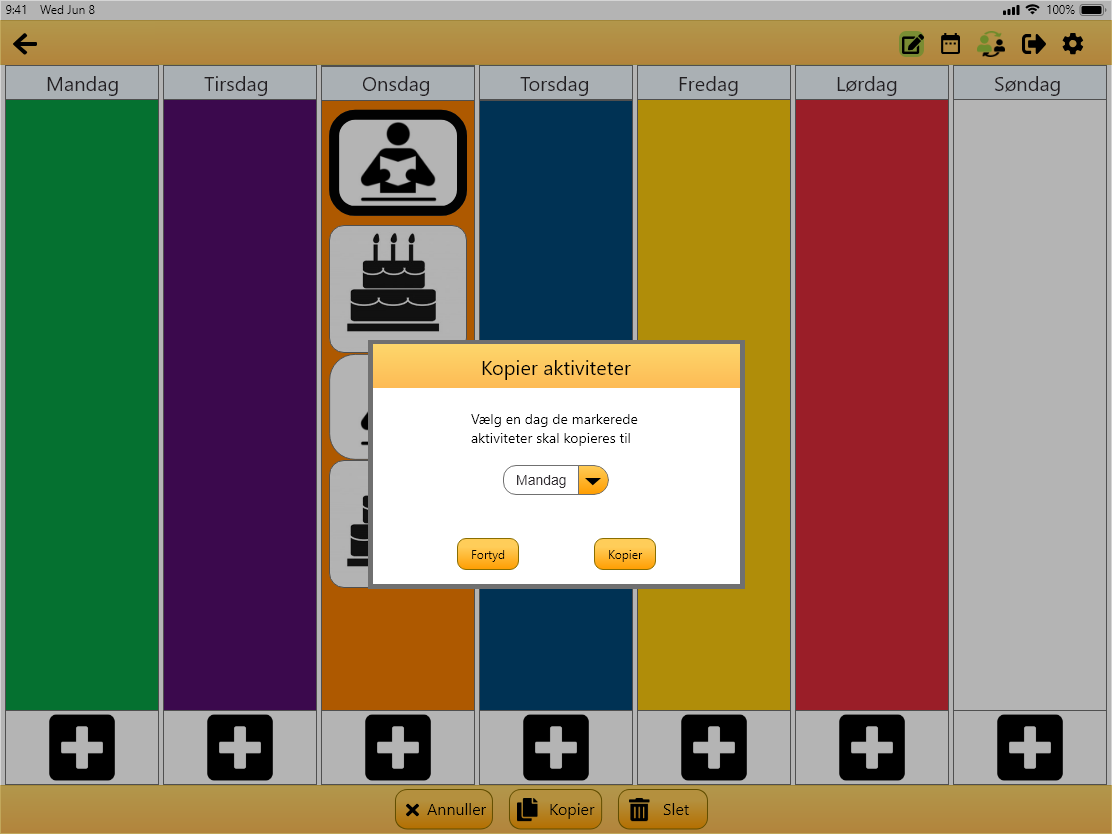
\includegraphics[width=1\linewidth, height=5cm]{mark_mode_copy_dropdown.png}
    \caption{Copy activities dialog with dropdown}
    \label{fig:mark_mode_copy_dropdown}
    \end{subfigure} 
    \caption{}
    \label{fig:mark_mode_copy_dropdown_and_checkbox}
\end{figure}



\subsection{Adding new pictograms}
The customer would like the option to add their own pictograms if they could not find the one they needed. They suggested being able to add from the gallery of the phone or tablet or by taking a picture directly. So we created a few prototypes this sprint that shows how this could work. First in \autoref{fig:pictogram_bottom_bar} we needed to create a way to go from the pictogram search to a screen where the user could choose pictures from their gallery.
A bottom bar with two buttons was enough for this. In \autoref{fig:pictogram_add_gallery} we see the prototype for the screen where you can add photos from the gallery, and enter a name for the pictogram.
\begin{figure}[H]
    \begin{subfigure}{0.5\textwidth}
    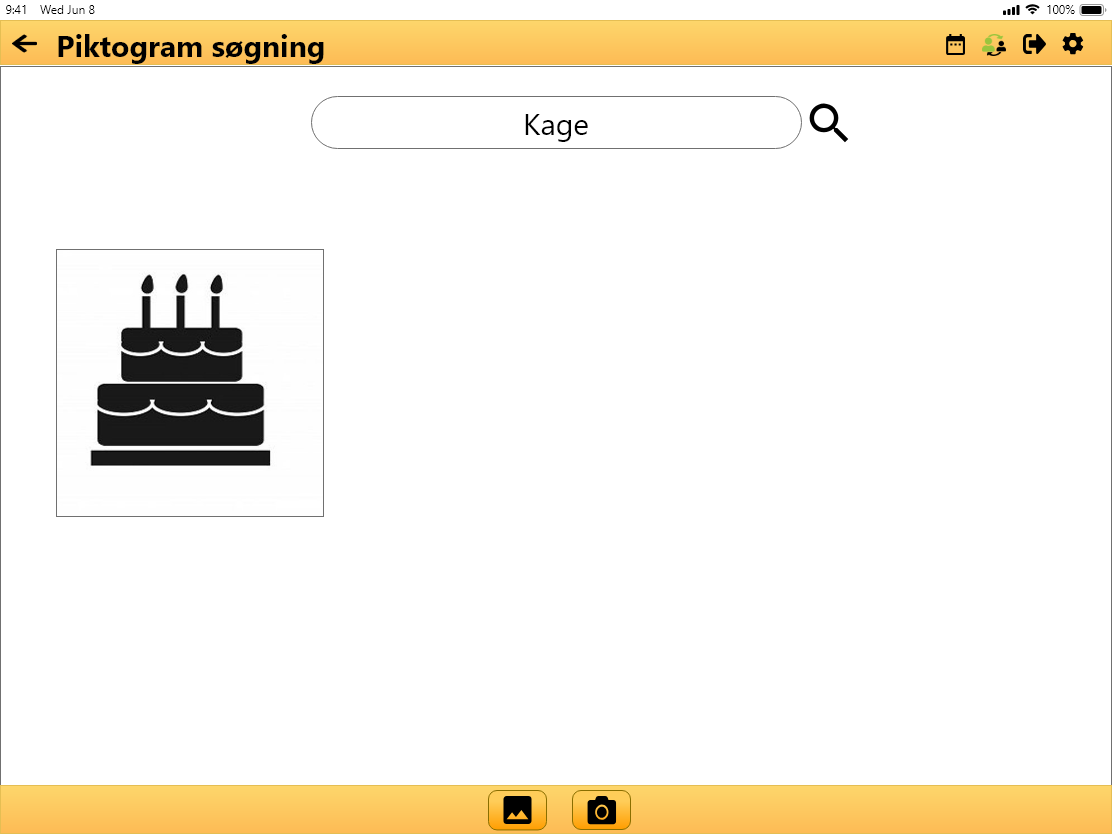
\includegraphics[width=1\linewidth, height=5cm]{pictogram_bottom_bar.png} 
    \caption{Pictogram search with options in the bottom bar}
    \label{fig:pictogram_bottom_bar}
    \end{subfigure}
    \begin{subfigure}{0.5\textwidth}
        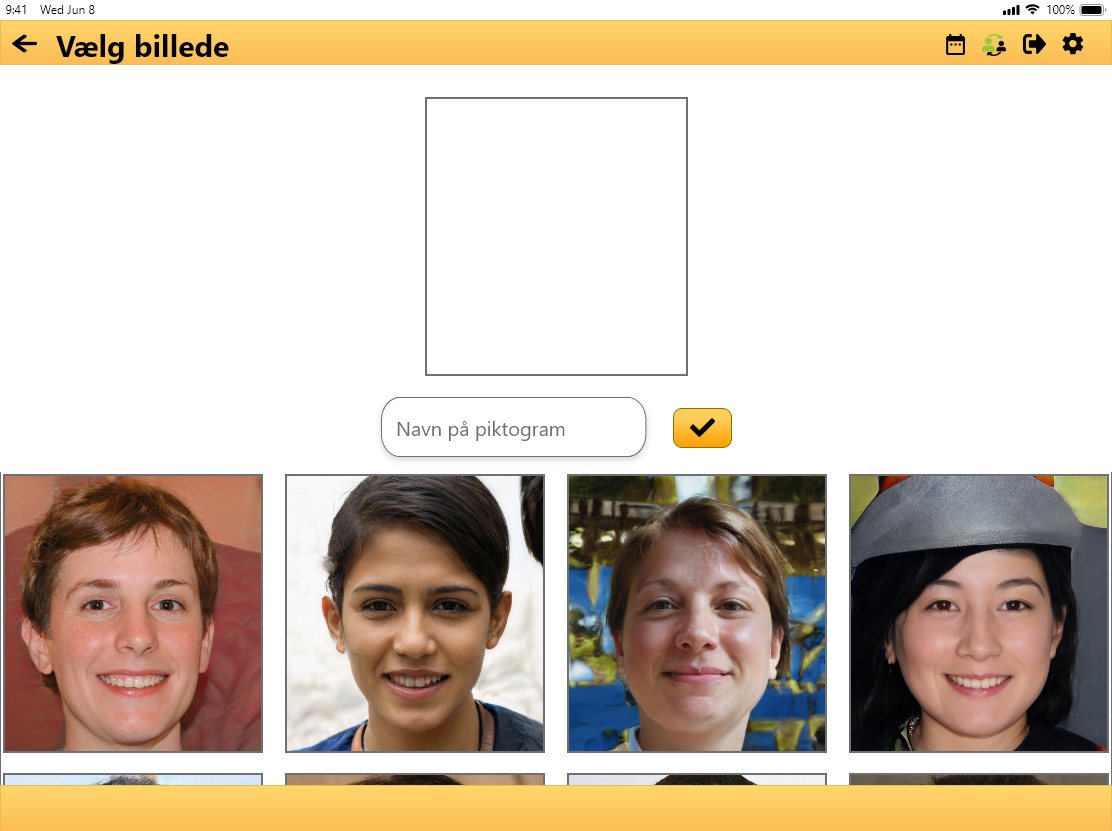
\includegraphics[width=1\linewidth, height=5cm]{pictogram_add_gallery.png}
    \caption{Screen for adding pictograms from gallery}
    \label{fig:pictogram_add_gallery}
    \end{subfigure} 
    \caption{}
    \label{fig:pictogram_bottom_bar_and_pictogram_add_gallery}
\end{figure}
\noindent
In \autoref{fig:pictogram_add_camera} we see the screen where the user can add a pictogram from the camera, give it name and then add it click the checkmark to save it to the week plan and in the database.

\begin{figure}
    \centering
    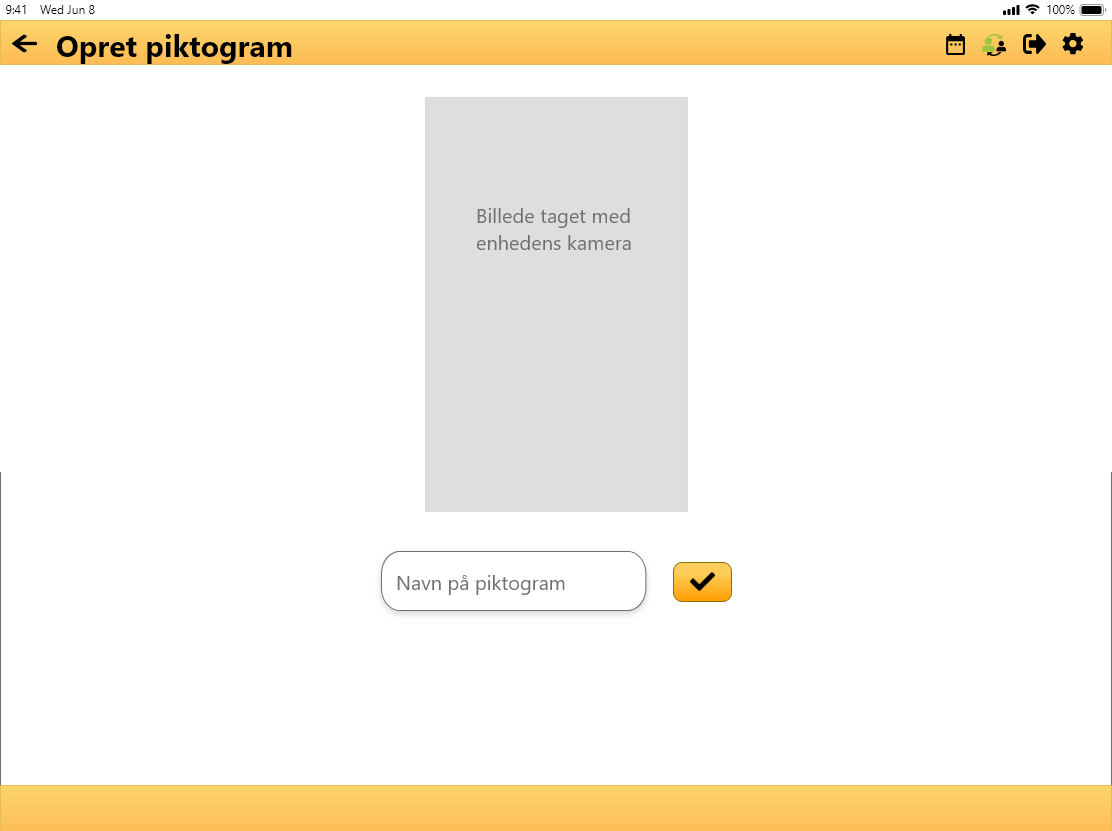
\includegraphics[width=0.5\linewidth]{pictogram_add_camera.png}
    \caption{Screen for adding pictogram by taking a picture with the device}
    \label{fig:pictogram_add_camera}
\end{figure}